%----------------------------------------------------------------------------------------------------------
% 	The following Latex code is given as an example and not The example
%	of using Latex to write report, memoir or thesis. 
%
%	Please visit the wikibook : https://fr.wikibooks.org/wiki/LaTeX
% 
%----------------------------------------------------------------------------------------------------------

\documentclass[11pt,a4paper]{article}

% package
%symbole math de l'American Mathematical Society (AMS)
\usepackage{amsfonts,amssymb,amsmath,amsthm}
\usepackage{systeme}
\usepackage{stmaryrd}
\usepackage{float}
%utiliser les regles de typographie francaise
\usepackage[french]{babel}
% accents 
%\usepackage[applemac]{inputenc} %MAC encoding
\usepackage[utf8]{inputenc} %UNIX encoding
%\usepackage[ansinew]{inputenc} %WINDOWS encoding

%graphique
\usepackage{color, graphicx, wrapfig, subcaption}

%citation
\usepackage{natbib}

\usepackage{tikz}
\usetikzlibrary{positioning}

%reference hypertext
\usepackage[pagebackref=false, hyperfootnotes=false]{hyperref}

%pour les url
\usepackage{url}
\urlstyle{sf}

%plusieur colonne dans tableau
% \multicolumn{nomb_col}{alignement}{contenu}
% \multirow{nomb_ligne}{largeur}{contenu}
\usepackage{multirow, multicol}

% layout
\usepackage[left=2cm, right=2cm, top=2.5cm, bottom=2.5cm]{geometry}

% les macros generales - exemples

%layout
\newcommand{\HRuleTop}{\noindent\rule{\linewidth}{.5pt}}
\newcommand{\HRuleBottom}{\rule{\linewidth}{.5pt}}
\newcommand{\ligne}{\rule[2mm]{.3\textwidth}{0.5mm}\\}
\newcommand{\myskip}{\vspace{\parskip}}
\newcommand{\blank}{ \clearpage{\pagestyle{empty}\cleardoublepage} }

%sets
\newcommand{\R}{\mathbb R}
\newcommand{\N}{\mathbb N}
\newcommand{\Z}{\mathbb Z}
\newcommand{\X}{\mathbb X}
\newcommand{\C}{\mathbb C}
\newcommand{\K}{\mathbb K}

\newcommand{\calN}{\mathcal N}
\newcommand{\calM}{\mathcal M}
\newcommand{\calA}{\mathcal A}
\newcommand{\calB}{\mathcal B}
\newcommand{\calE}{\mathcal E}
\newcommand{\calF}{\mathcal F}
\newcommand{\calL}{\mathcal L}
\newcommand{\calG}{\mathcal G}
\newcommand{\calP}{\mathcal P}
\newcommand{\calS}{\mathcal S}
\newcommand{\calU}{\mathcal U}
\newcommand{\barA}{\overline A}
\newcommand{\barV}{\overline V}

\newcommand{\bA}{\boldsymbol{A}}
\newcommand{\bB}{\boldsymbol{B}}
\newcommand{\bC}{\boldsymbol{C}}
\newcommand{\bD}{\boldsymbol{D}}
\newcommand{\bH}{\boldsymbol{H}}
\newcommand{\bL}{\boldsymbol{L}}
\newcommand{\bM}{\boldsymbol{M}}
\newcommand{\bN}{\boldsymbol{N}}
\newcommand{\bP}{\boldsymbol{P}}
\newcommand{\bQ}{\boldsymbol{Q}}
\newcommand{\bR}{\boldsymbol{R}}
\newcommand{\bT}{\boldsymbol{T}}
\newcommand{\bU}{\boldsymbol{U}}
\newcommand{\bX}{\boldsymbol{X}}

\newcommand{\bzero}{\boldsymbol{0}}
\newcommand{\be}{\boldsymbol{e}}
\newcommand{\bff}{\boldsymbol{f}}
\newcommand{\bI}{\boldsymbol{I}}
\newcommand{\bx}{\boldsymbol{x}}
\newcommand{\by}{\boldsymbol{y}}
\newcommand{\bz}{\boldsymbol{z}}
\newcommand{\bt}{\boldsymbol{t}}


%text style
\newcommand{\pkg}{\textbf}
\newcommand{\sigle}{\textsc}
\newcommand{\code}{\texttt}
\newcommand{\soft}{\textsf}
\newcommand{\expo}{\textsuperscript}

%_____________ avec couleur _____________ 
\newcommand{\cyan}[1]{{\color{cyan}#1}}
\newcommand{\red}[1]{{\color{red}#1}}
\newcommand{\blue}[1]{{\color{blue}#1}}



%math operator
\newcommand{\abs}[1]{\left\lvert#1\right\overt}
\newcommand{\bigo}[1]{\mathcal O \hskip -0.2em \left(#1\right)}
\DeclareMathOperator{\Ker}{Ker}
\newcommand{\littleo}[1]{o\hskip -0.2em \left(#1\right)}
\DeclareMathOperator{\mat}{mat}
\DeclareMathOperator{\rg}{rg}
\DeclareMathOperator{\sign}{sign}
\DeclareMathOperator{\Sp}{Sp}
\DeclareMathOperator{\Tr}{Tr}
\DeclareMathOperator{\vect}{vect}

\newtheorem*{definition}{Définition}
\newtheorem*{remark}{Remarque}
\newtheorem*{lemma}{Lemme}
\newtheorem*{theorem}{Théorème}

\title{Automate cellulaire probabiliste de l'électeur}
\author{%
Groupe 48 \\
\textsc{Chevallet} Django\;
\textsc{Cordonnier} Paul-Aliocha\;
\textsc{Maniak} Augustin\;
\textsc{Zenati} Racim
}


\begin{document}

\maketitle

\section{Introduction}

Nous nous intéressons ici aux automates cellulaires probabilistes dits
de l'électeur. Nous allons présenter ici le modèle
simple à deux valeurs possibles (0 ou 1) tel que formulé par
\cite{holley1975}.

Une chaîne de Markov est un processus aléatoire en temps discret dont 
l’évolution future ne dépend que de l’état présent, ce qui se traduit
par une matrice de transition stochastique décrivant les probabilités de 
passage entre états.

Soit $M$ la grille sur laquelle sont positionnées les particules. On a,
en dimension $d$, $N^d$ particules positionnées sur la grille $M =
\llbracket 1;N \rrbracket^d$. On se concentrera ici sur des valeurs de
$d$ appartenant à $\{1, 2, 3\}$. On note les particules voisines de
celle à la position $x \in M$ par $\mathcal{N}_x = \{ y \in M, ||y -
x||_d \leq 1, y \not= x\}$.

La valeur d'une particule évolue dans le temps (considéré discret et
représenté par un entier $n \in \mathbb{N}$).

Les particules ont une valeur comprise dans $\llbracket 0; \kappa
\rrbracket$. On a ici dans le modèle simple $\kappa = 1$. On
représente l'état de l'ensemble des particules par $\xi_n$ avec
$\xi_n(x)$ la valeur de la particule à la position $x$ à l'instant
$n$. On a $\xi_n \in \llbracket 0; \kappa\rrbracket^{N^d}$.

On a $\xi_{n + 1}(x) = i$ avec $i$ (appartenant à $\{0,1\}$)
choisi aléatoirement avec la
probabilité $p_x(i)$ suivante:

\[
\forall i \in \llbracket 0; \kappa\rrbracket, p_x(i) = \frac{\text{card}
  \{ y \in \mathcal{N}_x, \xi_n(y) = i \}}{\text{card }\mathcal{N}_x}
\]

Toutes les définitions données à partir de ce point dans cette section
proviennent de \cite{sericola2013}.

\begin{definition}[1.1]
    Un processus stochastique $X = \{X_n, n \in \mathbb{N}\}$ sur un espace d'états $S$ est une \textbf{chaîne de Markov à temps discret} si:
    \begin{equation*}
      \begin{split}
        &\forall n \geq 1,
        \forall X_0, \ldots, X_n \in S,
        \forall i_0, \ldots, i_n \in S, \\
        &\mathbb{P}\{X_n = i_n \mid X_{n-1} = i_{n-1}, \dots, X_0 =
        i_0\} = \mathbb{P}\{X_n = i_n \mid X_{n-1} = i_{n-1}\}
      \end{split}
    \end{equation*}
\end{definition}

La matrice de transition $P$ (souvent appelée matrice stochastique)
est une matrice carrée qui décrit la dynamique d'une chaîne de Markov
à temps discret sur un espace d'états fini. Chaque élément $P_{i,j}$
de la matrice représente la probabilité de transition de l'état $i$
vers l'état $j$ en une seule étape temporelle. Mathématiquement, elle
se définit par :
\begin{equation}
P_{i,j} = \mathbb{P}(\xi_{n+1} = j \mid \xi_n = i)
\end{equation}

Dans le cadre du modèle de l'électeur, l'espace d'états correspond à l'ensemble des configurations possibles des particules sur la grille, soit :
\begin{equation}
\xi_n \in \llbracket 0;\kappa\rrbracket^{N^d}
\end{equation}

La matrice doit vérifier les deux propriétés suivantes :
\begin{itemize}
    \item Tous ses coefficients sont positifs ou nuls ($P_{i,j} \ge 0$).
    \item La somme des probabilités de chaque ligne est égale à 1 ($\sum_{j} P_{i,j} = 1$), ce qui signifie qu'à partir d'un état donné, le système transite nécessairement vers un autre état (ou reste dans le même).
\end{itemize}

\begin{definition}[1.2]
    Une chaîne de Markov à temps discret $X = \{X_n, n \in \mathbb{N}\}$ sur un espace d'états $S$ est dite \textbf{homogène} si pour tout $n, k \in \mathbb{N}$ et pour tout $i, j \in S$, on a :
    \begin{equation*}
        \mathbb{P}\{X_{n+k} = j \mid X_k = i\} = \mathbb{P}\{X_n = j \mid X_0 = i\}
    \end{equation*}
\end{definition}

Soit $i$ un état de l'espace d'états. On définit le temps de premier retour vers l'état $i$, noté $T_i^+$, par la variable aléatoire:
\begin{equation}
T_i^+ = \inf \{ n \ge 1 \mid \xi_n = i \text{ sachant que } \xi_0 = i \}
\end{equation}


Il existe par ailleurs un lien fondamental entre le temps de retour et la loi stationnaire unique $\pi$:
\begin{equation}
\mathbb{E}[T_i^+] = \frac{1}{\pi_i}
\end{equation}

Pour tout état $i \in E$, on définit $f_{ii}^{(n)}$ comme la
probabilité que le premier retour à l'état $i$ se produise exactement
à l'instant $n$ et on note $f_{ii}$ la somme de ces probabilités sur
l'ensemble des instants:
\begin{equation}
f_{ii}^{(n)} = \mathbb{P}(\xi_n = i, \xi_{n-1} \neq i, \dots, \xi_1 \neq i \mid \xi_0 = i)
\end{equation}
\begin{equation}
f_{ii} = \sum_{n=1}^{\infty} f_{ii}^{(n)} = \mathbb{P}(T_i^+ < +\infty \mid \xi_0 = i)
\end{equation}

Cette quantité permet de caractériser la nature de l'état $i$ :
\begin{itemize}
    \item L'état $i$ est dit \textbf{récurrent} si et seulement si $f_{ii} = 1$ (le retour est certain).
    \item L'état $i$ est dit \textbf{transitoire} si et seulement si
      $f_{ii} < 1$ (il existe une probabilité non nulle de ne jamais
      revenir en $i$).
\end{itemize}

\begin{definition}[1.11]
  Une chaîne de Markov est dite \textbf{récurrente} (respectivement
  \textbf{transitoire}) si tous ses états sont récurrents
  (respectivement transitoires).
\end{definition}

\begin{definition}[1.12]
    Un état $i \in S$ est dit \textbf{absorbant} si $P_{i,i} = 1$.
\end{definition}

\begin{lemma}
Tout état absorbant est récurrent. En effet, si $i$ est un état
absorbant alors, par définition, on a $f_{i,i}^{(n)} =
\mathbf{1}_{\{n=1\}}$ et donc $f_{i,i} = 1$, c'est-à-dire que l'état
$i$ est récurrent.
\end{lemma}

\begin{theorem}[1.1]
  Pour une chaîne de Markov ergodique (irréductible et récurrente
  positive), la moyenne temporelle d'une fonction des états converge
  presque sûrement, quand le temps tend vers l'infini, vers sa
  moyenne spatiale par rapport à la loi stationnaire π.

  En d'autres termes, cela signifie qu'une seule trajectoire
  suffisamment longue de l'automate permet de retrouver les propriétés
  statistiques globales de tout le système (\cite{holley1975}).
\end{theorem}


\section{Problèmes en dimension $d = 1$}

On se place pour tous ces problèmes dans la condition $d = 1$.

\paragraph{Puissances de la matrice de transition.}

Soit $(X_n)_{n\geq 0}$ une chaîne de Markov de matrice $P$.
\[
\forall (i, j) \in S^2, \forall n \geq 0,
(P^{n})_{ij}
    = \mathbb{P}(X_n = j \mid X_0 = i)
\]
Ainsi, la matrice $P^n$ donne directement les probabilités de transition en $n$ pas.
Cette propriété est centrale pour analyser les lois en temps $n$ et les probabilités 
d'absorption dans les chaînes absorbantes.


\subsection{Cas de $N = 2$ à bords opposés}

\paragraph{Lien entre probabilité stationnaire et temps de retour.}

Pour une chaîne de Markov finie, irréductible et positivement récurrente,
la mesure stationnaire $\pi$ est unique et vérifie, pour tout état $i$ :
\[
\pi_i = \frac{1}{\mathbb{E}[T_i^{+}]}
\]
où $T_i^{+}$ est le temps de retour à $i$ :
\[
T_i^{+} = \inf\{n \ge 1 : X_n = i \mid X_0 = i\}
\]

Cela exprime que, sur une trajectoire longue, l'état $i$ est visité en moyenne
une fois tous les $\mathbb{E}[T_i^{+}]$ pas, ce qui correspond exactement à la
proportion de temps passée dans $i$, donc à $\pi_i$.


On a dans ce cas les états de grille suivants. Les conditions de bord
sont immuables.

\begin{figure}[h]
  \begin{center}
    \begin{tabular}{l | c | c c | c}
      état \\
      \hline
      A & 0 & 0 & 0 & 1 \\
      B & 0 & 0 & 1 & 1 \\
      C & 0 & 1 & 0 & 1 \\
      D & 0 & 1 & 1 & 1 \\
    \end{tabular}
  \end{center}
  \caption{États de grille possibles pour $N = 2$ à bords opposés}
\end{figure}

La chaîne de Markov correspondant à cette grille a pour matrice de
transition $P$ tel que suit:

\[
P = \begin{bmatrix}
  1/2 & 1/2 & 0 & 0 \\
  1/4 & 1/4 & 1/4 & 1/4 \\
  1/2 & 1/2 & 0 & 0 \\
  0 & 1/2 & 0 & 1/2 \\
\end{bmatrix}
\]

On observe directement qu'aucun état n'est absorbant, la chaîne de
Markov est donc irréductible sur l'espace d'état. Cette chaîne étant
finie et irréductible, le temps d'atteinte de chaque état est fini
donc pour tout état $x$ de l'espace d'états, $\pi(x) > 0$
(\cite{delmas2010}). Tous les états sont récurrents positifs, la
chaîne admet donc une loi stationnaire unique.

\begin{definition}
  Une probabilité $\pi$ sur la grille d'états d'une chaîne de Markov
  de matrice de transition $P$ est stationnaire si $\pi = \pi P$ (\cite{delmas2010}).
\end{definition}

On cherche donc le vecteur $\pi = [\pi_0, \pi_1, \pi_2, \pi_3]$ tel que
$\pi = \pi P$. On résout pour ça le système linéaire associé à ce
produit-équation de matrices:

\begin{equation}
  \begin{split}
    \systeme*{
      \pi_0 = \frac{1}{2}\pi_0 + \frac{1}{4}\pi_1 + \frac{1}{2}\pi_2,
      \pi_1 = \frac{1}{2}\pi_0 + \frac{1}{4}\pi_1 + \frac{1}{2}\pi_2 +
      \frac{1}{2}\pi_3,
      \pi_2 = \frac{1}{4}\pi_1,
      \pi_3 = \frac{1}{4}\pi_1 + \frac{1}{2}\pi_3
    }
    &\Longleftrightarrow
    \systeme*{
      \pi_0 = \frac{1}{2}\pi_1 + \pi_2,
      \pi_1 = \frac{2}{3}(\pi_0 + \pi_2 + \pi_3),
      \pi_2 = \frac{1}{4}\pi_1,
      \pi_3 = \frac{1}{2}\pi_1
    } \\
    &\Longleftrightarrow
    \systeme*{
      \pi_0 = \frac{3}{4}\pi_1,
      \pi_1 = \pi_1,
      \pi_2 = \frac{1}{4}\pi_1,
      \pi_3 = \frac{1}{2}\pi_1
    }
  \end{split}
\end{equation}

Or, on sait aussi que $\pi_0 + \pi_1 + \pi_2 + \pi_3 = 1$. On reformule donc
cela $(\frac{3}{4} + 1 + \frac{1}{4} + \frac{1}{2})\pi_1 = 1
\Longleftrightarrow \frac{5}{2}\pi_1 = 1$. On obtient ainsi le vecteur
suivant $\pi = [0.3; 0.4; 0.1; 0.2]$.

{\bfseries
En utilisant le lien entre probabilité stationnaire et temps de retour
formulé au dessus, on estime empiriquement le temps de retour moyen de
façon algorithmique de la manière suivante: sur un grand nombre ($m =
1000000$) d'itérations, on compte le nombre de fois qu'un même état
est rencontré et on estime à partir de ce nombre l'espérance du temps
de retour et ainsi la mesure stationnaire pour chaque état.
On trouve par cette méthode $\pi' = [0.22; 0.44; 0.11; 0.22]$, soit
une proportion plus faible que la proportion théorique pour l'état A
et ce indépendamment de l'état de départ choisi.
}

\subsection{Cas de $N = 2$ à bords égaux}

On a dans ce cas les états de grille suivants. Les conditions de bord
sont immuables.

\begin{figure}[h]
  \begin{center}
    \begin{tabular}{l | c | c c | c}
      état \\
      \hline
      A & 1 & 0 & 0 & 1 \\
      B & 1 & 0 & 1 & 1 \\
      C & 1 & 1 & 0 & 1 \\
      D & 1 & 1 & 1 & 1 \\
    \end{tabular}
  \end{center}
  \caption{États de grille possibles pour $N = 2$ à bords égaux}
\end{figure}

On représente l'automate probabiliste correspondant à ces conditions:

\begin{figure}[H]
  \begin{center}
    \begin{tikzpicture}[-latex, auto, node distance = 4cm, on grid,
        state/.style = { circle, draw }
      ]
      \node[state] (A) {A};
      \node[state] (B) [above right = of A] {B};
      \node[state] (C) [below right = of B] {C};
      \node[state] (D) [below left = of C] {D};

      \path (A) edge [loop left] node[left] {$1/4$} (A);
      \path (A) edge [bend left] node[left] {$1/4$} (B);
      \path (A) edge [bend right] node[left] {$1/4$} (C);
      \path (A) edge [bend right] node[left] {$1/4$} (D);
      \path (B) edge [bend left] node[left] {$1/2$} (C);
      \path (B) edge [bend right] node[left] {$1/2$} (D);
      \path (C) edge [bend left] node[left] {$1/2$} (B);
      \path (C) edge [bend left] node[left] {$1/2$} (D);
      \path (D) edge [loop below] node[left] {$1$} (D);
    \end{tikzpicture}
  \end{center}
  \caption{Automate probabiliste pour $N = 2$ à bords égaux}
\end{figure}

On voit directement que l'état $D$ est absorbant, étant donné que sa
seule transition est vers lui-même avec une probabilité de 1.

On agrège les configurations en trois états :
$A = (0,0),
B = \{(0,1),(1,0)\},
C = (1,1)$
avec $C$ absorbant.
La matrice de transition agrégée est :
\[
P =
\begin{pmatrix}
\frac14 & \frac12 & \frac14 \\
0 & \frac12 & \frac12 \\
0 & 0 & 1
\end{pmatrix}.
\]

Soit $T_i$ le temps d'absorption lorsque la chaîne part de $i$.
Les équations de première étape donnent:
\[
\begin{cases}
t_A = 1 + \frac14 t_A + \frac12 t_B\\[4pt]
t_B = 1 + \frac12 t_B
\end{cases}
\]
On résout et on trouve les temps d'absorption moyens suivants:
\[
\boxed{t_A = \frac{8}{3} \approx 2.67, \qquad t_B = 2}
\]

On peut aussi montrer que $t_B$ suit une loi géométrique de paramètre
1/2.  On se place dans l’état $B$. D’après la matrice de transition
agrégée, on a $\mathbb P(B \to C)=\tfrac12, \mathbb P(B \to
B)=\tfrac12$.  Ainsi, à chaque pas de temps, la chaîne reste en $B$
avec probabilité $\tfrac12$ ou est absorbée en $C$ avec probabilité
$\tfrac12$.

On note
$
T_B = \inf\{n \ge 1 : X_n = C \mid X_0 = B\}
$
le temps d’absorption lorsque la chaîne part de $B$.  
Pour que $T_B = n$, il faut que la chaîne reste en $B$ pendant $n-1$ itérations, 
puis passe de $B$ à $C$ à l’itération $n$. On obtient donc
\[
\mathbb P(T_B = n) = \left(\tfrac12\right)^{n-1}\tfrac12
\]
Ainsi, $T_B$ suit une loi géométrique de paramètre $\tfrac12$.
L’espérance du temps d’absorption vaut alors
\[
\mathbb E[T_B] = \frac{1}{\tfrac12} = 2
\]
ce qui donne le temps moyen d’absorption lorsque la chaîne part de l’état $B$.
À l'aide d'une simulation algorithmique (moyenne pour $m = 10000$
répétitions), on estime les temps d'absorption suivants: 2,65 pour
$A$ et 1,99 pour $B$, soit des valeurs très proches de
ce qui est obtensible par la théorie.

\subsection{Cas de $N = 3$}

On représente ci-dessous la matrice de transition correspondant au cas
$N=3$.  Les deux états absorbants sont $(0,0,0)$ et $(1,1,1)$, les
autres états étant transitoires.  On considère que les conditions au
bord sont périodiques, ie. que le voisin de gauche de la particule de
la première colonne est la particule de la dernière colonne et
inversement pour la particule de la dernière colonne.

\[
P =
\begin{pmatrix}
1 & 0 & 0 & 0 & 0 & 0 & 0 & 0\\
0 & 1 & 0 & 0 & 0 & 0 & 0 & 0 \\
\frac 14 & 0 & 0 & 0 & 0 & \frac 14 & \frac 14 & \frac 14 \\
0 & \frac 14 & 0 & 0 & \frac 14 & 0 & \frac 14 & \frac 14 \\
0 & \frac 14 & 0 & \frac 14 & 0 & \frac 14 & \frac 14 & 0 \\
\frac 14 & 0 & \frac 14 & 0 & \frac 14 & 0 & 0 & \frac 14 \\
0 & \frac 14 & \frac 14 & \frac 14 & \frac 14 & 0 & 0 & 0 \\
\frac 14 & 0 & \frac 14 & \frac 14 & 0 & \frac 14 & 0 & 0 \\
\end{pmatrix}
\]

On observe bien les deux états absorbants sur les lignes 1 et 2 avec un unique 1 sur la diagonale.

Les simulations montrent que pour un état initial comportant deux
zéros (resp. deux un), la chaîne de Markov est absorbée
par (0,0,0) (resp. (1,1,1)) avec une probabilité voisine de 2/3,
l’autre état absorbant n’étant atteint qu’avec une probabilité
d’environ 1/3.


\subsection{Cas de $N = 4$}

On représente ci-dessous un automate probabiliste simplifié pour le
cas $N = 4$ avec conditions périodiques.  Contrairement au cas $N =
3$, la dynamique fait apparaître trois classes absorbantes : les états
homogènes $(0,0,0,0)$ et $(1,1,1,1)$, ainsi qu’une classe
absorbante cyclique formée des configurations alternées $(0,1,0,1)$ et
$(1,0,1,0)$.  Les autres états de l’espace d’états sont transitoires
et rejoignent presque sûrement l’une de ces trois classes.

À partir de l’automate programmé de manière déterministe, nous
simulons l’évolution du système en choisissant aléatoirement l’état
initial (hors classes absorbantes), puis en itérant l’automate jusqu’à
absorption, avec une borne $n = 100000$.  Sur $m = 10000$ simulations,
les probabilités d’absorption obtenues sont d’environ $0{,}226$ pour
$(0,0,0,0)$, $0{,}310$ pour $(1,1,1,1)$, et respectivement $0{,}231$
et $0{,}234$ pour les états alternés $(0,1,0,1)$ et $(1,0,1,0)$.  On
constate ainsi que, contrairement au cas $N = 3$ où la dynamique
converge uniquement vers des états homogènes, le cas $N = 4$ favorise
également l’émergence d’un motif périodique stable.

\paragraph{Périodicité.}
Soit $i$ un état de la chaîne de Markov.
On définit d’abord l’ensemble des temps de retour possibles en $i$ par
$
\mathcal{N}(i)=\{\,n \ge 1 \;:\; \mathbb{P}(X_n = i \mid X_0 = i) > 0\,\}
$.
Cet ensemble regroupe tous les instants auxquels il est possible de
revenir à l’état $i$ avec une probabilité strictement positive.  La
période de l’état $i$ est alors définie par
$d(i)=pgcd(\mathcal{N}(i))$. Elle correspond au plus grand diviseur
commun des temps de retour possibles et mesure la régularité avec
laquelle la chaîne peut revisiter l’état $i$.

Dans notre cas, on observe une transition déterministe $0101\to 1010$
et $1010\to 0101$ avec probabilité $1$.  Ainsi, en partant de $0101$,
un retour en $0101$ n'est possible qu'après un nombre pair
d'itérations : $\mathbb{P}(X_{2}=0101\mid X_0=0101)=1$ tandis que
$\mathbb{P}(X_{2k+1}=0101\mid X_0=0101)=0$.  On en déduit que
$d(0101)=2$ (et de même $d(1010)=2$), et que la classe $\{0101,1010\}$
est une classe récurrente périodique de période $2$.
\\

\begin{remark}
L’automate présenté ci-dessous est une version simplifiée de la chaîne
de Markov complète.  L’espace d’états total comporte 16 configurations
possibles, mais seules les plus représentatives sont affichées : les
trois classes absorbantes (0000, 1111 et la classe périodique \{0101,
1010\}) ainsi que quelques états transitoires typiques.  De même,
seules les transitions principales et les probabilités associées
issues du code sont représentées : les transitions vers des états non
affichés ou celles provenant d’états qui admettent 16 transitions
équiprobables ont été omises afin de préserver la lisibilité du
schéma.
\end{remark}

\begin{figure}[H]
  \begin{center}
    \begin{tikzpicture}[
        -latex,
        auto,
        on grid,
        state/.style = {circle, draw, minimum size=9mm},
        every node/.style={font=\small}
      ]

      % --- Position des états (fixée pour éviter les croisements) ---
      % Ligne du haut : composantes absorbantes
      \node[state] (A) at (0,0)   {0000};  % 0000 (0)
      \node[state] (C) at (3,1.5) {0101};  % 0101 (5)
      \node[state] (D) at (6,1.5) {1010};  % 1010 (10)
      \node[state] (B) at (9,0)   {1111};  % 1111 (15)

      % Ligne du bas : quelques états transitoires
      \node[state] (E) at (3,-1.5) {0001}; % 0001 (1)
      \node[state] (F) at (6,-1.5) {0010}; % 0010 (2)
      \node[state] (G) at (9,-3)   {0111}; % 0111 (7)
      \node[state] (H) at (3,-3)   {1011}; % 1011 (11)

      % --- Boucles sur les états absorbants ---
      \path (A) edge [loop left, looseness=6]  node[left]  {$1$} (A);
      \path (B) edge [loop right, looseness=6] node[right] {$1$} (B);

      % Cycle périodique {C,D}
      \path (C) edge [bend left=15]  node[above] {$1$} (D);
      \path (D) edge [bend left=15]  node[below] {$1$} (C);

      % --- Transitions depuis E = 0001 (état 1)
      % next_state(1) : choix uniforme parmi {0,2,8,10}
      \path (E) edge[bend left=12]  node[left]  {$\tfrac14$} (A); % -> 0000
      \path (E) edge               node[right] {$\tfrac14$} (F); % -> 0010
      \path (E) edge[bend left=18] node[above] {$\tfrac14$} (D); % -> 1010

      % --- Transitions depuis F = 0010 (état 2)
      % next_state(2) : choix uniforme parmi {0,1,4,5}
      \path (F) edge[bend left=10] node[right] {$\tfrac14$} (A); % -> 0000
      \path (F) edge               node[below] {$\tfrac14$} (E); % -> 0001
      \path (F) edge[bend left=15] node[above] {$\tfrac14$} (C); % -> 0101

      % --- Transitions depuis G = 0111 (état 7)
      % next_state(7) : choix uniforme parmi {10,11,14,15}
      \path (G) edge[bend left=15] node[right] {$\tfrac14$} (D); % -> 1010
      \path (G) edge[bend left=15] node[right] {$\tfrac14$} (H); % -> 1011
      \path (G) edge[bend left=25] node[right] {$\tfrac14$} (B); % -> 1111

      % --- Transitions depuis H = 1011 (état 11)
      % next_state(11) : choix uniforme parmi {5,7,13,15}
      \path (H) edge[bend left=15] node[left]  {$\tfrac14$} (C); % -> 0101
      \path (H) edge[bend left=15] node[left]  {$\tfrac14$} (G); % -> 0111
      \path (H) edge[bend left=25] node[left]  {$\tfrac14$} (B); % -> 1111

    \end{tikzpicture}
  \end{center}
  \caption{Automate probabiliste simplifié pour le cas $N=4$.}
\end{figure}

Les états A et B sont absorbants, C et D forment une composante
absorbante périodique et les autres états (y compris ceux qui ne sont
pas indiqués dans l'automate) sont transitoires.

\paragraph{Convergence exponentielle des chaînes de Markov finies.}

Pour une chaîne de Markov finie, homogène et irréductible, la
distribution en temps $n$, notée $\pi^{(n)}$, converge vers la
distribution stationnaire $\pi$ lorsque $n \to \infty$.  Cette
convergence est exponentielle au sens suivant : si $Q$ est la matrice
de transition, alors pour un vecteur initial $\mu$, on a $\mu Q^n
\longrightarrow \pi \text{ quand } n \to \infty$ et l'écart $\|\mu Q^n
- \pi\|$ décroît approximativement comme $\lambda_2^n$, où $\lambda_2$
est la valeur propre de $Q$ ayant le deuxième plus grand module après
$1$.

Si $Q$ est diagonalisable, on peut écrire $Q = V \Lambda V^{-1}, \quad
Q^n = V \Lambda^n V^{-1}$, où $\Lambda$ est diagonale et contient
toutes les valeurs propres. Comme $\lambda_1 = 1$ correspond à la
distribution stationnaire, les contributions des autres valeurs
propres décroissent géométriquement avec $n$.

Ainsi, la vitesse de convergence vers l'état stationnaire est dictée
par $|\lambda_2|$.  Plus $|\lambda_2|$ est petit, plus la convergence
est rapide. Cette approche permet également de quantifier le temps de
mélange de la chaîne, ie. le nombre d'itérations nécessaires pour que
la distribution approche suffisamment $\pi$.

On obtient par une simulation numérique dans le cas d = 1, N = 2 à
bords opposés:
\begin{figure}[h]
  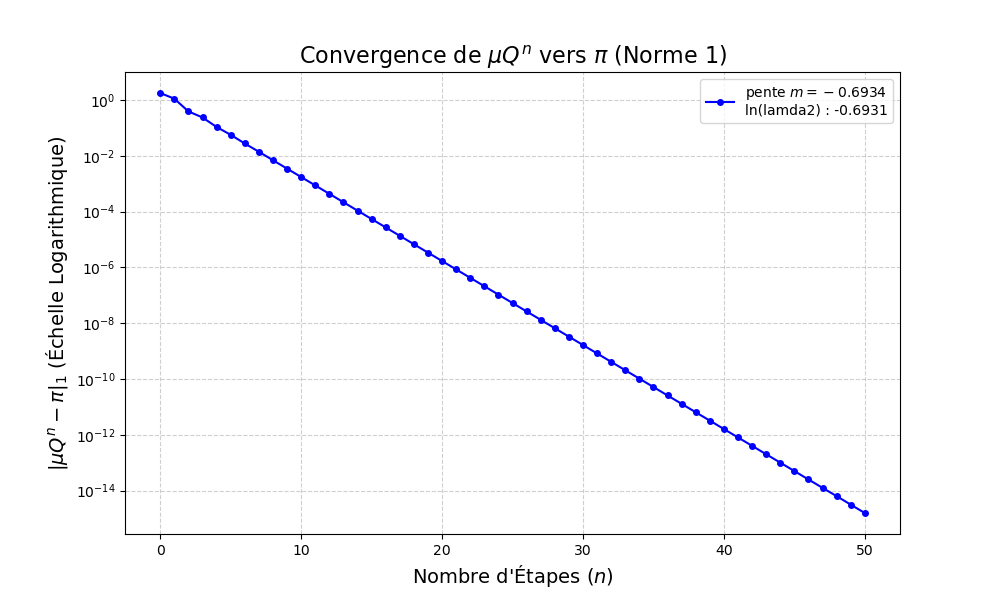
\includegraphics[width=\textwidth]{courbe_cv_exp}
  \caption{Simulation de convergence vers $\pi$.}
\end{figure}

L'hypothése selon laquelle $\|\mu Q^n - \pi\|$ décroît comme $\lambda_2^n$ est alors numériquement validée.

\section{Dimension $d = 2$}

\subsection{Périodicité et configurations en damier}

Concernant la périodicité : lorsque l'on utilise le voisinage de von
Neumann en 2D, pour les grilles de taille paire (de côté $2k$), on
peut voir apparaître un damier parfait avec alternance 0/1. Chaque
cellule a quatre voisins et tous les voisins d'une cellule $0$ sont
des $1$ et vice-versa. Cette configuration peut former une classe
récurrente périodique de période $2$, où le damier se renverse à
chaque itération, générant un état bloquant alterné stable.

Pour les grilles de taille impaire (de côté $2k+1$), un damier
parfait n’est plus possible car les lignes et colonnes sont de
longueur impaire. Certaines cellules auront plus de voisins d’un type
que de l’autre, ce qui empêche de se retrouver dans une classe
récurrente périodique.  Les motifs alternés ne sont pas stables et la
chaîne finit par converger vers un état absorbant homogène (tout $0$
ou tout $1$), où la probabilité de convergence dépend de la
configuration initiale.  Ainsi, les motifs périodiques bloquants
apparaissent uniquement pour les grilles de taille paire tandis que
les états absorbants homogènes apparaissent sur toutes les grilles.

\subsubsection{Analyse pour le cas des bords fixés à 1}

Dans cette simulation, nous considérons des grilles initiales $5 \times 5$ entourées
d’un encadrement fixe de $1$, formant une grille effective $7 \times 7$.  
Le système évolue selon les règles probabilistes avec voisinage de von Neumann.

Les résultats montrent que toutes les simulations convergent vers l'état absorbant
tout-$1$, confirmant que les bords fixes dominent la dynamique.  
Le temps moyen d'absorption dépend légèrement de la configuration initiale : lorsque
la majorité de la grille centrale est initialement composée de $1$, l'absorption est plus
rapide ($\bar{T} \approx 2{,}18$ itérations), tandis qu'une majorité de $0$ ralentit
la convergence ($\bar{T} \approx 3{,}00$ itérations).

Cette différence illustre la sensibilité du temps de convergence à l'état initial,
tout en restant compatible avec la convergence exponentielle attendue d'une chaîne
de Markov finie vers son état absorbant unique.  
La présence d'un encadrement homogène fixe crée un biais net qui entraîne une absorption
rapide et systématique dans l'état tout-$1$, démontrant l’influence des conditions aux
bords sur la dynamique globale du système.

\subsubsection{Répartition périodique avec $N = 5$}

On observe par la simulation qu'en choisissant des grilles de taille
paire, l'automate finit par osciller entre des états alternants (états damiers).

Pour des grilles de taille impaire, ici $5 \times 5$, et en effectuant
$10\,000$ simulations, on obtient un temps d'absorption moyen de
$46{,}83$ étapes et lorsqu'une opinion est dominante dans l'état
initial, l'état absorbant (ici dit de consensus) sera une grille
constituée uniquement de cette opinion dominante dans plus de la
moitié des cas ($57{,}84\%$).

\subsection{Influence du nombre d’opinions $\kappa \in \llbracket 3, n \rrbracket$}

On étudie ici l'influence du nombre d'opinions possibles $\kappa$ sur la dynamique de l'automate
cellulaire probabiliste défini sur une grille spatiale en dimension $2$
(voisinage de von Neumann), sur une grille centrale $5\times 5$.
Deux variantes de conditions aux bords sont considérées :
(i) bords périodiques (non fixés) et
(ii) bords fixés à une opinion constante $b \in \{0,\dots,\kappa-1\}$
via un encadrement externe homogène.

Pour chaque valeur de $\kappa$, nous réalisons $M=10\,000$ simulations
indépendantes.  On mesure le temps moyen d'absorption $\bar{T}$
jusqu'à atteindre un consensus homogène sur la grille centrale, et une
corrélation entre l'opinion dominante initiale et l'opinion finale de
consensus, définie comme la proportion de simulations pour lesquelles
l'opinion finale est égale à l'opinion majoritaire au temps initial.

\paragraph{Cadre markovien (cas $\kappa \ge 3$)}

Soit $\Lambda$ l’ensemble des sites de la grille centrale $N\times N$
(ici $N=5$).  L’espace d’états est
$\mathcal{S}=\{0,\dots,\kappa-1\}^{\Lambda}$ avec
$|\mathcal{S}|=\kappa^{N^2}$. À l’instant $n$, l’état du système est
la configuration globale $\xi_n \in \mathcal{S}$.

Pour tout site $x\in\Lambda$ et toute opinion $c\in\{0,\dots,\kappa-1\}$, on note
\[
p_x^{(n)}(c)=\frac{1}{|\mathcal{N}_x|}\sum_{y\in\mathcal{N}_x}\mathbf{1}_{\{\xi_n(y)=c\}}
\]
où $\mathcal{N}_x$ désigne l’ensemble des voisins de von Neumann de $x$ (avec la convention
de bord choisie). La règle d’évolution est $\mathbb{P}\big(\xi_{n+1}(x)=c \mid \xi_n\big)=p_x^{(n)}(c)$.

\begin{lemma}
  Pour toute paire de configurations $\eta,\eta'\in\mathcal{S}$, la probabilité
  de transition de $\eta$ vers $\eta'$ ne dépend que de $\eta$ :
  \[
  \mathbb{P}(\xi_{n+1}=\eta' \mid \xi_n=\eta,\xi_{n-1},\dots,\xi_0)
  =\mathbb{P}(\xi_{n+1}=\eta' \mid \xi_n=\eta).
  \]
  Ainsi, $(\xi_n)_{n\ge 0}$ est une chaîne de Markov.
  Elle est \emph{homogène} car la règle de mise à jour (donc la matrice de transition)
  ne dépend pas de $n$.
\end{lemma}

\subsubsection{États absorbants et rôle des conditions aux bords.\\}

\paragraph{Cas des bords non fixés}
Pour toute opinion $c\in\{0,\dots,\kappa-1\}$, on définit la configuration constante
$\xi^{(c)}\in\mathcal{S}$ par $\forall x\in\Lambda, \xi^{(c)}(x)=c$.

\paragraph{Preuve d'absorbance}

Si $\xi_n=\xi^{(c)}$, alors pour tout site $x$, tous ses voisins $y\in\mathcal{N}_x$
vérifient $\xi_n(y)=c$, donc
\[
p_x^{(n)}(c)=\frac{1}{|\mathcal{N}_x|}\sum_{y\in\mathcal{N}_x}\mathbf{1}_{\{\xi_n(y)=c\}}=1.
\]
Ainsi, pour tout $x\in\Lambda$, $\mathbb{P}(\xi_{n+1}(x)=c\mid
\xi_n)=1$ et par conséquent $\mathbb{P}(\xi_{n+1}=\xi^{(c)}\mid \xi_n=\xi^{(c)})=1$,
c’est-à-dire que $\xi^{(c)}$ est un état absorbant.

\paragraph{Cas des bords fixés}
On impose un encadrement externe constant d’opinion $b$ (les sites du bord valent $b$ à tout instant).
On ne fait évoluer que la grille centrale $\Lambda$.
La configuration centrale homogène ``tout-$b$'' (i.e. $\xi^{(b)}$ sur $\Lambda$) est absorbante :
si $\xi_n=\xi^{(b)}$, alors chaque site central voit uniquement des voisins d’opinion $b$
(les voisins internes valent $b$ et les voisins du bord sont fixés à $b$),
donc $p_x^{(n)}(b)=1$ et $\xi_{n+1}=\xi^{(b)}$ p.s.

\paragraph{Existence d’une classe fermée}
Comme $\mathcal{S}$ est fini, la chaîne admet au moins une classe récurrente fermée
(théorème général des chaînes de Markov finies : toute chaîne finie se décompose en états transitoires
et classes récurrentes fermées). En particulier, l’existence d’au moins un état absorbant implique
l’existence d’au moins une classe fermée non vide.

\subsubsection{Conséquences qualitatives et validation numérique.\\}

\paragraph{Bords non fixés : effet de $\kappa$}

Quand les bords ne sont pas fixés, la dynamique consiste en une compétition entre opinions.
Un argument simple permettant de \emph{quantifier} l’effet de $\kappa$ est la probabilité qu’un site
subisse une mise à jour fortement polarisée.

Supposons l’état initial tiré uniformément dans $\mathcal{S}$ (indépendance site à site).
Pour un site $x$, les opinions de ses $4$ voisins sont i.i.d. uniformes sur $\{0,\dots,\kappa-1\}$.
Alors :
\[
\mathbb{P}(\text{les 4 voisins ont la même opinion})
=\sum_{c=0}^{\kappa-1}\mathbb{P}(\text{voisins tous = }c)
=\kappa\left(\frac{1}{\kappa}\right)^4=\frac{1}{\kappa^3}.
\]
Or, dans ce cas, la mise à jour en $x$ est déterministe (probabilité $1$ d’adopter cette opinion).
Cette probabilité $\frac{1}{\kappa^3}$ décroît rapidement quand $\kappa$ augmente : les mises à jour
``quasi-déterministes'' deviennent rares.

De plus, la probabilité d’observer une \emph{majorité stricte} parmi les 4 voisins (au sens 3--1 ou 4--0)
se calcule explicitement :
\begin{equation*}
  \begin{split}
\mathbb{P}(\text{majorité stricte})
=\mathbb{P}(4\text{ égaux})+\mathbb{P}(3\text{ égaux})
=\frac{1}{\kappa^3}+\kappa(\kappa-1)\binom{4}{3}\left(\frac{1}{\kappa}\right)^4
=\frac{1}{\kappa^3}+\frac{4(\kappa-1)}{\kappa^3}
&=\frac{4\kappa-3}{\kappa^3} \\
&= \mathcal{O}(\frac{1}{\kappa^2})
  \end{split}
\end{equation*}

Donc cette probabilité est de l’ordre de $1/\kappa^2$ (faible dès que $\kappa\ge 3$),
ce qui signifie que les mises à jour sont plus souvent ``diffuses'' (2--2 ou 2--1--1, etc.),
ralentissant la coalescence des domaines et augmentant typiquement les temps d’absorption.

Dans notre cas ($\kappa=3$, grille $5\times5$), on obtient numériquement
$\bar{T}\approx 56{,}17$ itérations, ce qui est cohérent avec la raréfaction des voisinages
très polarisés quand $\kappa$ augmente.

\paragraph{Bords fixés : biais vers l'opinion imposée}

Lorsque les bords sont fixés à $b$, l’encadrement injecte en permanence l’opinion $b$ dans le système.
On peut formaliser un \emph{biais minimal local} :

Soit $x$ un site de la grille centrale adjacent au bord (c’est-à-dire ayant au moins un voisin sur le bord).
Alors au moins un voisin de $x$ vaut $b$, donc
\[
p_x^{(n)}(b)=\frac{\text{card}\{y\in\mathcal{N}_x:\xi_n(y)=b\}}{4}\ge \frac{1}{4}.
\]

On a donc $\mathbb{P}(\xi_{n+1}(x)=b\mid \xi_n)\ge \frac{1}{4}$.  Ce
\emph{flux de probabilité} non nul, réinjecté à chaque pas, favorise
l’apparition de sites à $b$ au bord puis la croissance d’un domaine de
valeur $b$ vers l’intérieur (mécanisme de propagation).  On s’attend
donc à une diminution nette du temps moyen d’absorption et une baisse
de la corrélation ``état final = dominante initiale'' lorsque la dominante
initiale est différente de $b$.

Expérimentalement, pour $\kappa=3$ et une grille $5\times5$ avec bords fixés,
on observe $\bar{T}\approx 16{,}8$, nettement inférieur au cas non fixé.
De plus, la corrélation dépend de $b$ :
avec bord fixé à $b=2$, on observe $2871/10000$ corrélations,
tandis qu'avec bord fixé à $b=0$, on observe $3779/10000$ corrélations,
ce qui s’explique par l’interaction entre la majorité initiale et l’opinion imposée au bord.




\section{Conclusions}\label{conclusions}

Nous avons étudié l’automate cellulaire probabiliste de l’électeur
comme une chaîne de Markov homogène sur un espace d’états fini
$\mathcal S=\{0,\dots,\kappa-1\}^{\Lambda}$, ce qui garantit
l’existence de classes récurrentes fermées et permet une analyse en
termes d’absorption, de récurrence et de périodicité. En dimension
$1$, l’écriture explicite de la matrice de transition pour des petites
tailles (dont $N=2$) permet de déterminer rigoureusement les lois
stationnaires et/ou les temps d’absorption via des équations de
premier pas, avec une validation numérique en accord avec les valeurs
théoriques.

Pour $N=3$ et $N=4$ en dimension $1$, l’étude des classes absorbantes
met en évidence l’apparition de phénomènes qualitatifs nouveaux :
au-delà des états homogènes absorbants, des classes récurrentes
périodiques peuvent exister (période $2$ pour le cycle
$\{0101,1010\}$), ce qui illustre le rôle de la structure du voisinage
et des symétries dans la décomposition de l’espace d’états.

En dimension spatiale $2$, nous avons montré que les configurations
homogènes sont absorbantes, et que les conditions aux bords modifient
profondément la dynamique. Sans bords fixés, l’augmentation du nombre
d’opinions $\kappa$ réduit la probabilité de voisinages fortement
polarisés (par exemple $\mathbb{P}(\text{4 voisins
  égaux})=1/\kappa^3$), ce qui ralentit la coalescence des domaines et
augmente les temps moyens d’absorption. À l’inverse, un encadrement
externe constant impose un biais minimal non nul vers l’opinion $b$ au
voisinage du bord (au moins $1/4$ pour un site adjacent), accélérant
fortement l’absorption et diminuant la corrélation entre majorité
initiale et consensus final lorsque la majorité initiale diffère de
$b$.

Ainsi, ce travail met en évidence comment la finitude (cadre
markovien), la géométrie (dimension et parité de la grille) et les
conditions aux bords gouvernent la nature des classes récurrentes
(absorbantes ou périodiques) et les temps caractéristiques de
convergence, et comment les simulations permettent d’illustrer et de
corroborer ces propriétés sur des instances de taille modérée.


%%%%%%%%%%%%%%%%%%%%%%%%%%%%%%%%%%%%%%%%%%%%
%  Bibiliography.
%%%%%%%%%%%%%%%%%%%%%%%%%%%%%%%%%%%%%%%%%%%%
\bibliographystyle{agsm}  
\phantomsection %add a phantom section for the hyperreference linkg
\addcontentsline{toc}{section}{Bibliographie} %add a chapter to the TOC
\bibliography{biblio}   %must have a file named biblio.bib

\end{document}
